\documentclass[14pt]{extarticle} 
\usepackage{unicode-math}
\usepackage{amsthm,graphicx,xcolor,natbib,enumitem,booktabs,tabularx}
%\usepackage[paperwidth=126mm, paperheight=96mm, top=5mm, bottom=5mm, right=5mm, left=5mm]{geometry}
\usepackage[margin=1cm]{geometry}
\pagenumbering{gobble}

\usepackage[BoldFont,SlantFont]{xeCJK}  
\xeCJKsetemboldenfactor{2}
\setCJKmainfont{cwTeX Q Yuan Medium}

\newcommand{\ds}{\displaystyle}
\newcommand{\ie}{\,\Longrightarrow\,}
\newcommand{\ifff}{\,\Longleftrightarrow\,}
\newcommand{\mi}{\mathrm{i}}
\DeclareMathOperator*{\dom}{dom}
\DeclareMathOperator*{\codom}{codom}
\DeclareMathOperator*{\ran}{ran}
\newcommand{\floor}[1]{\lfloor #1 \rfloor}
\newcommand{\ceil}[1]{\lceil #1 \rceil}

% figure --> 圖
\renewcommand{\appendixname}{附錄}
\renewcommand{\figurename}{圖}
\renewcommand{\tablename}{表}
\renewcommand{\refname}{參考文獻}

\usepackage{hyperref}
\hypersetup{
    colorlinks,
    linkcolor={red!50!black},
    citecolor={blue!60!black},
    urlcolor={blue!60!black}
    %urlcolor={blue!80!black}
}

\theoremstyle{definition}
\newtheorem*{dfn}{定義}
\newtheorem*{prp}{性質}
\newtheorem*{thm}{定理}
\newtheorem*{ex}{例}
\newtheorem*{sol}{解}
\newtheorem*{prf}{證}

%\setenumerate{label=(\roman*),itemsep=1pt,topsep=3pt}
\newcommand{\myline}{\noindent\makebox[\linewidth]{\rule{\paperwidth}{0.4pt}}}
%\newcommand{\myline}{\textcolor[RGB]{220,220,220}{\rule{\linewidth}{1pt}}}

\usepackage{tikz}
\usetikzlibrary{arrows.meta,angles,quotes}
\usepackage{pgfplots}
% axis style, ticks, etc
\pgfplotsset{every axis/.append style={
                   label style={font=\fontsize{4}{4}\selectfont},
                   tick label style={font=\fontsize{4}{4}\selectfont}  
               },
            }
\renewcommand\tabularxcolumn[1]{m{#1}}

\begin{document}
\title{\texorpdfstring{\vspace{-1em} 畢氏定理證明}{畢氏定理證明}} 
\author{\vspace{-3em}}
\date{\vspace{-3em}}

\maketitle

\begin{thm}[畢氏定理(Pythagorean Theorem)]
  直角三角形 $\Delta ABC$ 如圖,則 $c^2 = a^2 + b^2$。 
\end{thm}

\begin{prf}
  \begin{figure}[!htbp]
    \centering
    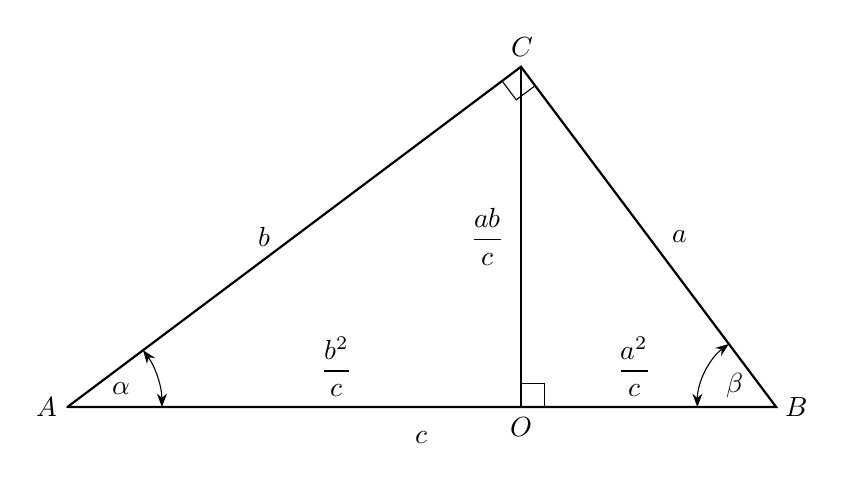
\begin{tikzpicture}[scale=1.8, >={Stealth[scale=1]}]
      \draw (0, 0) node[left] {$A$};
      \draw (16 / 5, 0) node[below] {$O$};
      \draw (5, 0) node[right] {$B$};
      \draw (16 / 5, 12 / 5) node[above] {$C$};
      \draw (41 / 10 + 0.1, 6 / 5) node[right] {$a$};
      \draw (8 / 5 - 0.1, 6 / 5) node[left] {$b$};
      \draw (2.5, -0.1) node[below] {$c$};
      \draw (16 / 5 - 0.05, 6 / 5) node[left] {$\ds\frac{ab}{c}$};
      \draw (8 / 5 + 0.3, 0) node[above] {$\ds\frac{b^2}{c}$};
      \draw (16 / 5 + 8 / 10, 0) node[above] {$\ds\frac{a^2}{c}$};
      \draw[thick] (0, 0) -- (5, 0) -- (16 / 5, 12 / 5) -- (0, 0);
      \draw (16 / 5, 0) -- (16 / 5, 12 / 5);
      \draw (5, 0) coordinate (a) -- (16 / 5, 0) coordinate (b) -- (16 / 5, 12 / 5) coordinate (c) pic [draw,angle radius=3mm] {right angle = a--b--c};
      \draw (5, 0) coordinate (a) -- (16 / 5, 12 / 5) coordinate (b) -- (0, 0) coordinate (c) pic [draw,angle radius=3mm] {right angle = a--b--c};
      \draw (16 / 5, 0) coordinate (a) -- (0, 0) coordinate (b) -- (16 / 5, 12 / 5) coordinate (c) pic ["$\alpha$",draw,<->,angle radius=12mm] {angle = a--b--c};
      \draw (16 / 5, 12 / 5) coordinate (a) -- (5, 0) coordinate (b) -- (16 / 5, 0) coordinate (c) pic ["$\beta$",draw,<->,angle radius=10mm] {angle = a--b--c};
    \end{tikzpicture}
  \end{figure}

  \begin{itemize}
    \item[]
    \item 由直角三角形面積公式 
      \begin{align*}
        \frac{1}{2}\,c\cdot\overline{CO} = \frac{1}{2}\,a\cdot b\ie\overline{CO} = \frac{ab}{c}
      \end{align*}
    \item 由三角形相似關係
      \begin{align*}
        \Delta ABC\sim\Delta CBO\sim\Delta ACO
      \end{align*}
      則 
      \begin{align*}
        &\overline{AC}:\overline{BC} = \overline{CO}:\overline{BO} = \overline{AO}:\overline{CO} \\
        \ie& b:a = \frac{ab}{c}: \overline{BO} = \overline{AO}: \frac{ab}{c} \\
        \ie& \overline{BO} = \frac{a^2}{c},\;\overline{AO} = \frac{b^2}{c}
      \end{align*}
    \item 由圖
      \begin{align*}
        \overline{AB} = \overline{AO} + \overline{BO} \ie c = \frac{b^2}{c} + \frac{a^2}{c}\ie c^2 = a^2 + b^2
      \end{align*}
  \end{itemize}
\end{prf}
  
\end{document}
